\documentclass[11pt,a4paper,twocolumn]{article}
% Mahmood Amintoosi, http://amintoosi.blogspot.com
% m.amintoosi@gmail.com
% این فایل و فایلهای ضمیمه‌ی آن از سایت www.parsilatex.com قابل برداشت هستند.
% محمود امین طوسی - دانشگاه علم و صنعت ایران 
% این مقاله در هفدهمین کنفرانس مهندسی برق ایران در اردیبهشت ۸۸ ارائه شده است.

% شما می‌توانید از این فایل به عنوان یک الگو برای مقالات خود استفاده نمایید.

% برای پردازش پس از یکبار استفاده از xelatex با استفاده از دستور زیر لیست مراجع را تولید نمایید:
% bibtex (F11 در TexStudio)
% و سپس دوبار استفاده از xelatex. (یعنی همان Quick Build در Texmaker یا TexStudio را دوبار بزنید.)


% تمام بسته های مورد نیاز برای ایجاد یک مقاله به صورت کامل اینجا آورده شده است در صورتی که بخواهید از بسته های دیگر استفاده کنید بهتر است که انها را به گونه ای انتخاب کنید که با این بسته ها تداخل نداشده باشد. نکته این که به نظر من استفاده از همین بسته ها کافی است.
\usepackage{amsthm,amssymb,amsmath}

\usepackage{setspace}
% اگر بخواهید چند شکل را در کنار همدیگر داشته باشید، از این بسته استفاده می‌کنیم.
\usepackage{subfigure}
\usepackage{algorithm}
\usepackage{algorithmic}
% در این قالب از بسته graphx برای انجام کارهای گرافیکی استفاده می‌شود. این بسته
% برای اضافه کردن تصویرها به متن استفاده شده است.
\usepackage{graphicx}

% برای تنظیم حاشیه صفحات
\usepackage[top=25mm, bottom=25mm, left=20mm, right=20mm]{geometry}

\setlength{\columnwidth}{82mm}
\setlength{\columnsep}{6mm}

% بسته ای برای رنگی کردن لینک ها و فعال سازی لینک ها در یک نوشتار، بسته hyperref باید جزو آخرین بسته‌هایی باشد که فراخوانی می‌شود. 
\usepackage[pagebackref =true,colorlinks=true]{hyperref}

\usepackage{xepersian}


%%%%%%%%%%%%%%%%%%%%%%%%%%%%%%%%%%%%%%%%%%%%%%%%%%%%%%%%%%%%%%%%%%%%%%
%  تنظیم اندازه فونت ها،

\settextfont[Scale=1]{B Nazanin}
\setlatintextfont[Scale=.9]{Times New Roman}
%\setdigitfont{XB Zar}

\defpersianfont\NazaninBold[Scale=1]{B Nazanin Bold}
\defpersianfont\AbstractBold[Scale=.92]{B Nazanin Bold}
%%  با استفاده از این دستور می‌توان فونت و فارسی و یا انگلیسی بودن اعداد در فرمول‌ها را به حالت اولیه (یعنی پیش‌فرض لاتک) برگرداند.
\DefaultMathsDigits
% حذف عبارت چکیده
\renewcommand{\abstractname}{}

% اختصاص - به عنوان جداکننده شماره بخش و زیربخش
\SepMark{-}

% به صورت پیش‌فرض بعد از شماره بخش - نداریم، مگر آنکه شماره زیر بخش پس از آن آمده باشد. از آنجا که مطابق قالب کنفرانس در هر صورت
% پس از شماره بخش و شماره زیربخش به جداکننده نیاز داریم از دستورات زیر استفاده می‌کنیم:
\makeatletter
\renewcommand \thesection {\@arabic\c@section\@SepMark}
\renewcommand \thesubsection {\thesection\@arabic\c@subsection\@SepMark}
\makeatother

% تغییر نام algorithm به الگوریتم
\floatname{algorithm}{الگوریتم}

\numberwithin{table}{section}
\onehalfspacing


% دستور لازم برای تعریف محیط lr برای این که بدون هیچ مشکلی بتوان در عنوان فصل و یا بخش انگلیسی نوشت
\makeatletter
\let\orig@lr\lr
\renewcommand*{\lr}[1]{\texorpdfstring{\orig@lr{#1}}{#1}}
\makeatother

% با دستور زیر اندازه فرمولها را تغییر می‌دهیم. این دستور با فونت اندازه ۱۲ به خوبی کار می‌کند ولی با فونت اندازه ۱۱ که دراین مقاله استفاده نموده‌ام که ۶ صفحه بیشتر نشود، مشکلاتی دارد. به سایت: زیر مراجعه فرمایید: http://www.latex-community.org/forum/viewtopic.php?f=5&t=1792
\DeclareMathSizes{10.95}{9.2}{7.3}{5.5} %12,10,8,6

\thispagestyle{empty}

% برای اینکه چکیده حاشیه نداشته باشد
\renewcommand\abstract{}



\begin{document}


\title{\vspace{13mm}\NazaninBold{
ثبت تصویر مبتنی بر شباهت ساختاری تصاویر با کاربرد در
}}
\author{
محمود امین‌طوسی، محمود فتحی و ناصر مزینی\\
دانشگاه علم و صنعت ایران، دانشکده مهندسی کامپیوتر\\
\lr{\small\{mAmintoosi,mahFathy,Mozayani\}@iust.ac.ir}
}

%%%%%%%%
% برخی دستورات زیر برای آن گذاشته شده‌اند که چکیده به صورت تک ستونی باشد اگر می‌خواهید که قسمت چکیده تک ستونه باشد، این کامنتهای زیر و کامنت %\end{@twocolumnfalse}] را بردارید. 
%\twocolumn[
%\begin{@twocolumnfalse}
\date{}
\maketitle

\begin{abstract}
\AbstractBold
{
\vspace{-5mm}
چکیده -
روش لوکاس-کاناد از جمله معروف‌ترین روش‌های ثبت تصویر مبتنی بر ناحیه است که گونه‌های مختلفی از آن تاکنون ارائه شده است. هدف اصلی در روشهای مختلف ثبت تصویر پیدا کردن پارامترهای مدل تبدیل، برای نگاشت دقیق یک تصویر بر روی مختصات تصویر دیگر است. در الگوریتم لوکاس-کاناد این امر از طریق کمینه‌سازی یک تابع مشخص کننده‌ی میزان تفاوت یک تصویر و تبدیل شده‌ی دیگری حاصل می‌شود. معمولاً تابع مذکور مربع تفاضلات بین دو تصویر در نظر گرفته می‌شود. در این مقاله از معیار شباهت ساختاری دو تصویر به عنوان ضریبی برای این تابع استفاده شده است. نحوه‌ی لحاظ کردن این معیار شباهت در فرمولبندی الگوریتم لوکاس-کاناد به صورت ریاضی بیان شده است. کمینه‌سازی مورد نظر با استفاده از شیوه‌ی بهینه‌سازی لونبرگ-مارکورت انجام شده است. نتایج پیاده‌سازی‌های انجام شده برتری شیوه‌ی پیشنهادی را در مقایسه با الگوریتم اصلی لوکاس-کاناد (با روشهای کمینه‌سازی گوس-نیوتن و لونبرگ-مارکورت) از نقطه نظر سرعت همگرائی نشان می‌دهد. همچنین کارائی شیوه‌ی پیشنهادی در مسئله‌ی وضوح برتر در مقایسه با چند روش دیگر نشان داده شده است.}
 \end{abstract}
{کلید واژه‌ها}-  ثبت تصویر، لونبرگ-مارکورت، موجک، وضوح برتر.\\
%\end{@twocolumnfalse}]
% حذف شماره صفحات
%\pagestyle{empty}

\section{مقدمه}
یکی از  مهمترین مسائل در حوزه‌ی پردازش تصویر و بینائی ماشین  ثبت تصویر می‌باشد. هدف از  پیدا کردن تبدیل مناسب بین دو یا چند تصویر از یک صحنه است. در حالت کلی، باید تناظری یکتا بین یک نقطه از یک تصویر و نقطه‌ای دیگر از تصویر دوم  به نحوی پیدا نمود که هر دو نشان‌دهنده‌ی یک نقطه از صحنه باشند. 
 مسئله‌  قرابت نزدیکی با مسائل  تخمین حرکت و دیگر مسایل 

اخیراً نویسندگان در \cite{Amintoosi08reconstruction,Amintoosi09regional} شیوه‌ای مشتمل بر استفاده از تصاویر آموزشی با وضوح بالا را برای افزایش وضوح تصویر ورودی ارائه نموده‌اند؛ در مقالات فوق‌الذکر مواردی مورد لحاظ قرار نگرفته است که در این مقاله به موارد زیر پرداخته خواهد شد:
\begin{enumerate}
\item
در \cite{Amintoosi08reconstruction} برای ثبت تصویر فقط از یک شیوه‌ی مبتنی بر ویژگی استفاده شده است، در حالیکه این شیوه همیشه نتایج دقیقی تولید نمی‌کند؛ در این مقاله شیوه‌ی ثبت تصویر لوکاس-کاناد با استفاده از معیار شباهت ساختاری دو تصویر $SSIM$\LTRfootnote{ Structural SIMilarity (SSIM)}\cite{Wang04image} بهبود داده شده و در شیوه‌ی ارائه شده در \cite{Amintoosi08reconstruction} بکار گرفته شده است؛
\item
در \cite{Amintoosi08reconstruction,Amintoosi09regional} مرحله‌ی همرنگ نمودن تصاویر مورد ترکیب، بدون درز نبوده است؛ در این مقاله با استفاده از روش  همرنگ‌سازی چند بانده این نقیصه برطرف شده است.
\end{enumerate}

 در بخش \ref{Sec:TheProposedMethod} شیوه‌ی پیشنهادی، در بخش \ref{Sec:ExperimentalResults} نتایج پیاده‌سازی‌ها و در انتها جمع‌بندی آورده شده است.




\section{شیوه‌ی پیشنهادی}\label{Sec:TheProposedMethod}

در شیوه‌ی پیشنهادی برای وضوح برتر توسط نگارندگان در \cite{Amintoosi08reconstruction}، هر یک از تصاویر باوضوح بالا، به عنوان تصویر آموزشی، متناظر با قسمتی از تصویرِ باوضوح پایین هستند.  تصاویر آموزشی می‌توانند تفاوتهایی با تصویر اصلی از نقطه نظر شدت روشنائی یا زاویه‌ی اخذ داشته باشند. 

 این تفاوتها می‌تواند ناشی از برداشت عکسها در زمانهای متفاوت و یا با دوربینهای متفاوت و از زوایای مختلف باشد. در این شیوه ابتدا تصویر با وضوح پایین به اندازه‌ی مطلوب بزرگ شده و سپس  تبدیل مناسبی برای نگاشت هر یک از تصاویر آموزشی بر روی تصویر مورد نظر با استفاده از  نقاط کلیدی \lr{SIFT}\LTRfootnote{ Scale Invariant Feature Transform (SIFT)} و الگوریتم \lr{RANSAC}\LTRfootnote{ RANdom SAmple Consensus (RANSAC)} در قالب ماتریس هوموگرافی پیدا می‌شود. در انتها تصویرِِ باوضوح بالای نگاشت شده، با تصویر باوضوح پایین ورودی  می‌شود.

چارچوب کلی کار در این مقاله در شکل~\ref{fig:OneLR_oneHR} آمده است. دو مرحله‌ی « دقیق‌تر نمودن مدل با استفاده از ثبت تصویر مبتنی بر ناحیه» و «همرنگ نمودن تصاویر در نواحی مرزی» در این مقاله اضافه شده‌اند. از آنجا که ذکر روش کار برای یک یا چند تصویر آموزشی تفاوتی ندارد، در اینجا فرض بر آن است که فقط از یک تصویر آموزشی استفاده می‌شود.

\begin{figure}
\centering 
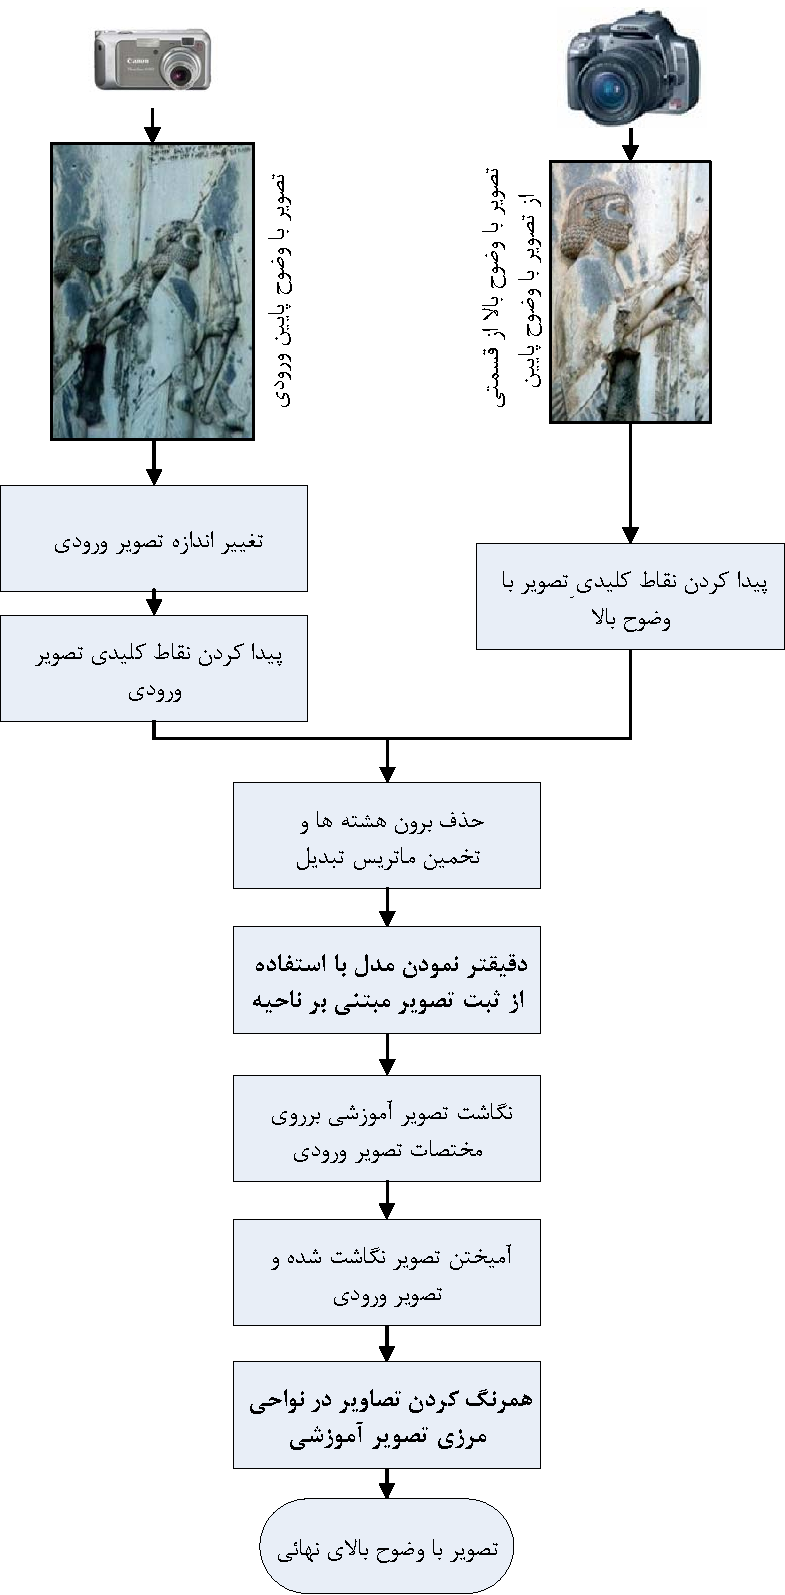
\includegraphics[width=70mm]{Images/OneLR_oneHR.pdf}
\caption{چارچوب کلی شیوه‌ی پیشنهادی.}
\label{fig:OneLR_oneHR}
\end{figure}


مهمترین قسمت در کار حاضر استفاده از معیار مقایسه‌ی ساختاری دو تصویر ($SSIM$) برای بهبود شیوه‌ی ثبت تصویر لوکاس-کاناد\cite{Lucas81iterative} می‌باشد. در مراجع از فرمولبندی‌های متفاوتی برای بیان این شیوه استفاده شده است. در این مقاله از فرمولبندی ذکر شده در \cite{Baker04lucas-kanade20part1} استفاده خواهیم نمود و لذا مروری بر این فرمولبندی ضروری می‌باشد که در ادامه ذکر خواهد شد. پس از آن نگاهی بر معیار مقایسه‌ی $SSIM$ داشته و سپس روش پیشنهادی بر اساس آنها بیان خواهد شد.
%
\subsection{الگوریتم لوکاس-کاناد}
هدف در شیوه‌ی ثبت تصویر لوکاس-کاناد\cite{Lucas81iterative} کمینه‌سازی مجموع مربع تفاضلات زیر بین تصویر آموزشیِ $T(\mathbf{x})$ و نگاشت تصویر ورودیِ $I(\mathbf{x})$ است:
 \begin{equation}\label{eq:SSD_L2Norm}
    SSD=\sum _x ^{W} H^{2} 
\end{equation}
که در آن $A$ بیانگر مدل تبدیل‌ (در اینجا پروجکتیو)، $\mathbf{p}=(p_1,\dots,p_8)^T$ پارامترهای مدل تبدیل،  نگاشت تصویر ورودی $I$ بر روی مختصات تصویر آموزشی $T$ و $\mathbf{x} =(x,y)^T$ مختصات یک پیکسل می‌باشد.
 کمینه‌سازی \eqref{eq:SSD_L2Norm} نسبت به $\mathbf{p}$ انجام می‌شود. 
در شیوه‌ی لوکاس-کاناد فرض بر آن است که در ابتدا تخمینی از مدل دردست بوده و در یک فرآیند تکراری این تخمین بهبود داده می‌شود؛
در هر دور ابتدا عبارت زیر بر اساس $\triangle\mathbf{p}$ کمینه شده:
\begin{equation}\label{eq:SSD_L2Norm_deltap}
\sum_x[I(\mathbf{W}(\mathbf{x;\mathbf{p+\triangle p}}))-T(\mathbf{x})]^2
\end{equation}
و سپس پارامترها بروزرسانی می‌شوند:
\begin{equation}
\mathbf{p}\leftarrow\mathbf{p+\triangle p}
\end{equation}
دو مرحله‌ی فوق تا مادامیکه الگوریتم همگرا نشده است تکرار خواهند شد. در فرآیند کمینه‌سازی، $\mathbf{\triangle p}$ به صورت زیر محاسبه می‌شود:

که در آن $H$، ماتریس هسین تقریبی\LTRfootnote{ Approximate Hessian Matrix}، به صورت زیر بدست می‌آید:
\begin{equation}\label{eq:Hessian}
    H = \sum _x I
\end{equation}
این مراحل در الگوریتم 
\begin{algorithm}
\caption{الگوریتم ثبت تصویر لوکاس-کاناد مبتنی بر بهینه‌سازی گوس-نیوتون \lr{(LK-GN)}.}
\label{alg1}
\begin{latin}
\textbf{Input}:
The reference image $I$ and template image $T$.\\
\textbf{Output}: Registration parameters
$\mathbf{p}=(p_1,\dots,p_n)^T$ as the warp model $W$.
\begin{algorithmic}[1]
\REPEAT
  \STATE Warp $I$ with $W$ to compute $IW$. 
  \STATE Compute the error image $T(x)-IW$ 
  \STATE Warp the gradient $\nabla I$ with $W$. \STATE Evaluate the Jacobian
    ${W}{p}$ at $(\mathbf{x;p})$. 
  \STATE Compute the steepest descent images $\nabla I{W}{p}$. 
  \STATE \label{line:Hessian} Compute the Hessian matrix using Equation 
    \eqref{eq:Hessian}. 
  \STATE Compute $[\nabla {W}{p}]^T$ and $[T(x)-IW]$ 
  \STATE \label{alg1:deltap} Compute $\triangle\mathbf{p}$ using Equation \eqref{eq:deltap} 
  \STATE Update the parameters $\mathbf{p}\leftarrow\mathbf{p}+\triangle\mathbf{p}$ 
\UNTIL{$||\triangle\mathbf{p}||\leq\epsilon$ or Reaching to Maximum Iteration allowed}
\end{algorithmic}
\end{latin}
\end{algorithm}

\onecolumn
\begin{@twocolumnfalse}
\begin{table}
\begin{tabular}{p{3cm}p{3cm}cc}
1 & 2 & 1 & 2\\\hline
1 & 2 & 1 & 2\\\hline
1 & 2 & 1 & 2\\\hline
\end{tabular}
\end{table}
\end{@twocolumnfalse}

\section{شبیه‌سازی}
\label{Sec:ExperimentalResults}
 در این شبیه‌سازی قصد داریم تا مقاومت روش پیشنهادی در برابر نویز را مورد بررسی قرار دهیم. در هر سیگنال به مقدار نصف ظرفیت، بیت اطلاعات درج می‌کنیم. نویز سفید گاوسی با میانگین صفر و انحراف استانداردهای مختلف، بین  $0$  تا $40$، به سیگنال اضافه می‌شود. مقدار $\alpha = 0.015$ قرار داده شده است. در یک شبیه‌سازی دیگر نیز، نویز یکنواخت با انحراف استاندارد {$0$} تا {$40$} نیز بر سیگنال اعمال می‌شود.  این حملات بر روی 77 سیگنال ویدئویی استاندارد انجام گرفته‌است. اندازه قالب‌های سه‌بعدی نیز همان‌طور که پیشتر ارایه شد، برابر $16 \times 16 \times 16$ قرار داده می‌شود. ن
 
  در این شبیه‌سازی قصد داریم تا مقاومت روش پیشنهادی در برابر نویز را مورد بررسی قرار دهیم. در هر سیگنال به مقدار نصف ظرفیت، بیت اطلاعات درج می‌کنیم. نویز سفید گاوسی با میانگین صفر و انحراف استانداردهای مختلف، بین  $0$  تا $40$، به سیگنال اضافه می‌شود. مقدار $\alpha = 0.015$ قرار داده شده است. در یک شبیه‌سازی دیگر نیز، نویز یکنواخت با انحراف استاندارد {$0$} تا {$40$} نیز بر سیگنال اعمال می‌شود.  این حملات بر روی 77 سیگنال ویدئویی استاندارد انجام گرفته‌است. اندازه قالب‌های سه‌بعدی نیز همان‌طور که پیشتر ارایه شد، برابر $16 \times 16 \times 16$ قرار داده می‌شودتایج شبیه‌سازی‌های مورد اشاره،  شکل‌ ‎\ref{fig:Errorblock}‎، نمایی از شبیه‌سازی انجام گرفته ....
\begin{figure}
\centering
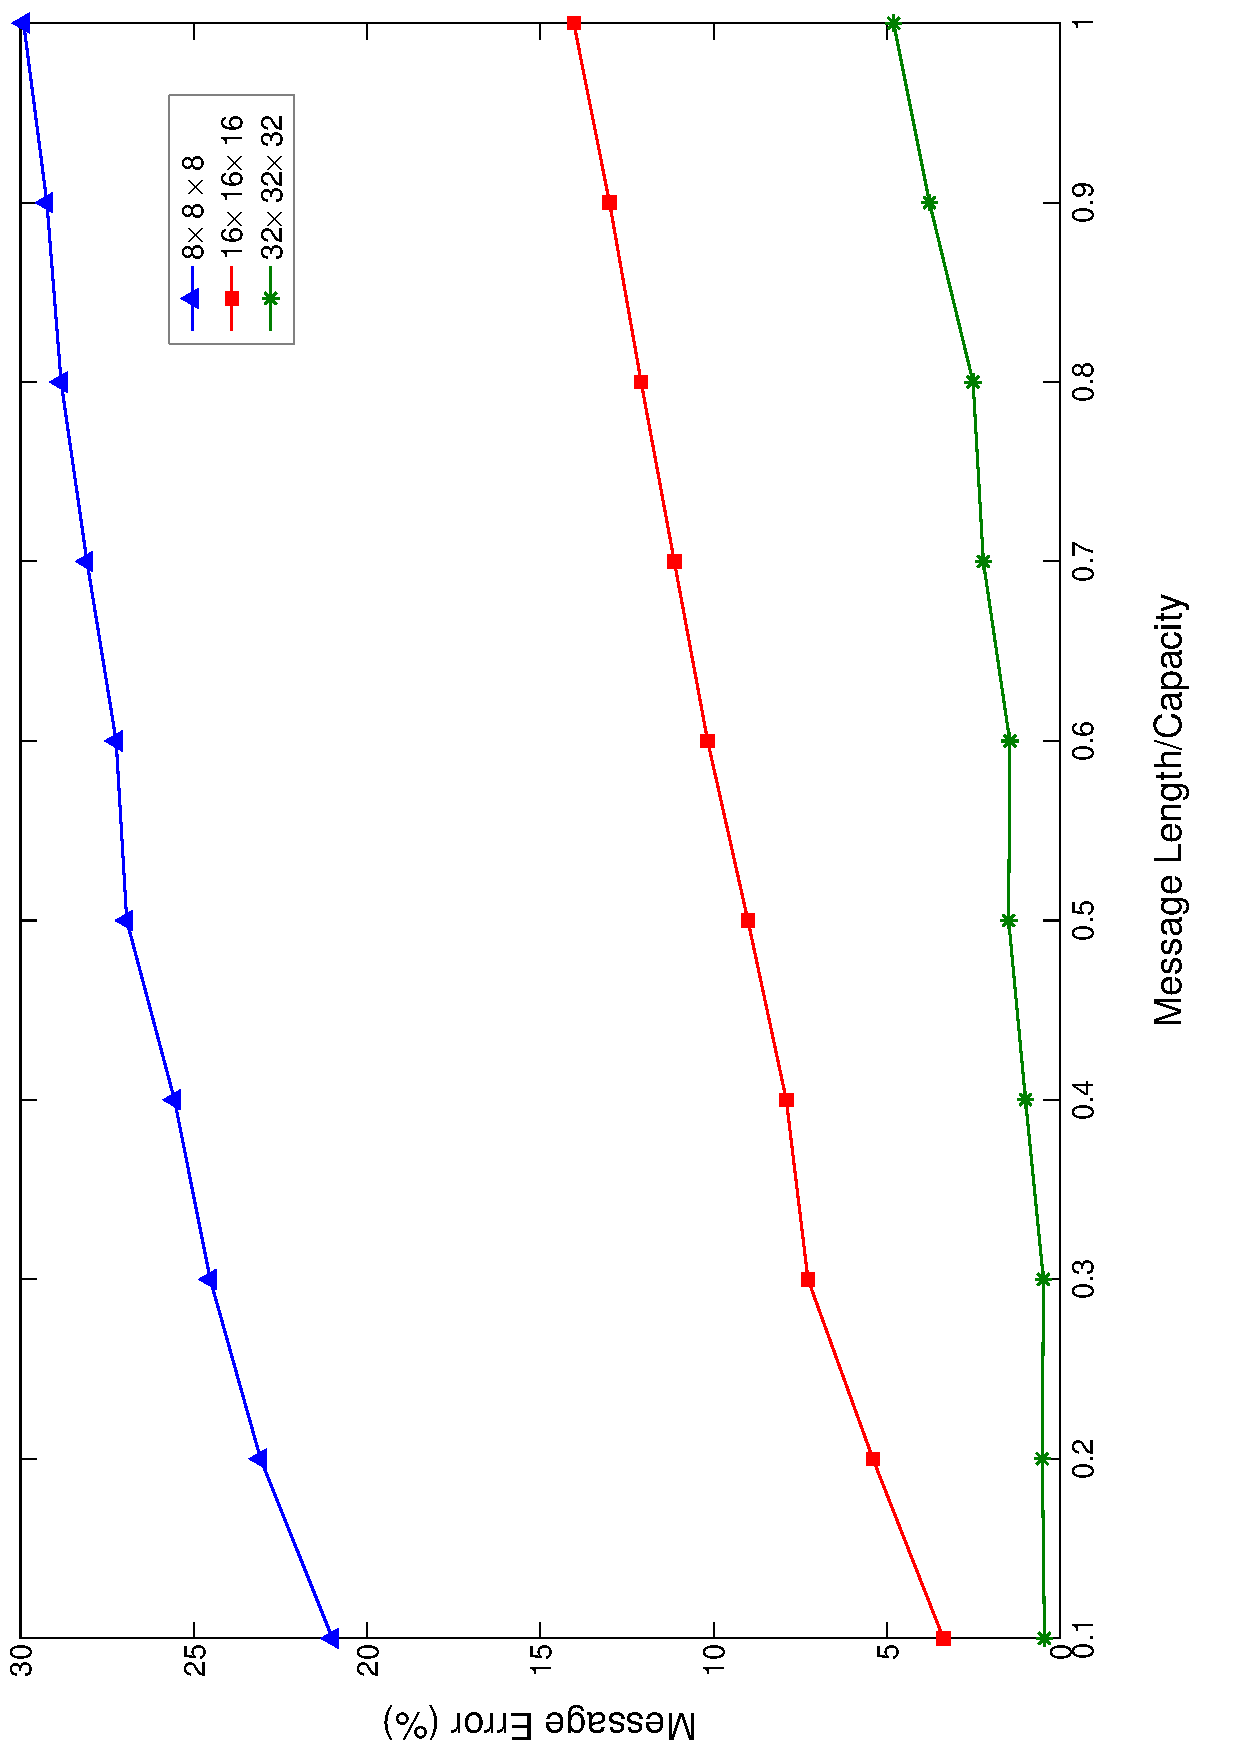
\includegraphics[width=0.7\linewidth,angle=270]{./Images/Errorblock}
\caption{
نمودار خطای تخمین به درصد برحسب نسبت طول پیام به کل ظرفیت
}
\label{fig:Errorblock}
\end{figure}


\section*{سپاس‌گزاری}
مؤلفین وظیفه‌ی خود می‌دانند که از آقای دکتر \lr{Peter Kovesi} بابت توابع سودمند \lr{MATLAB}  و آقایان وفا خلیقی، مصطفی واحدی و دکتر مهدی امیدعلی بابت زحمات و راهنمایی‌های ارزنده‌ی آنها در زمینه‌ی زی‌پرشین


%% سه دستور زیر باعث می‌شوند که مراجع با قلم کوچکتر و با فاصله خطوط کمتر و با فاصله بین مراجع کم ظاهر شوند. 
%% این حالت برای کاهش تعداد صفحات مقاله مناسب است.
%% می‌توانید هر یک از آنها را comment نموده و خروجی را ملاحظه فرمایید.
\small
\singlespacing
%%\setlength{\itemsep}{-1ex}


\renewcommand{\refname}{\rl{{مراجع}\hfill}}

\bibliographystyle{ieeetr-fa}
\bibliography{SR_References}


\end{document}


